%% Included in decks: design-handbook
\setSlideVersion{1-0-0}
\begin{standardframe}{Widgets: metadata and actions}
\begin{columns}[T,onlytextwidth]
\begin{column}{.48\linewidth}
\textbf{Light}\par
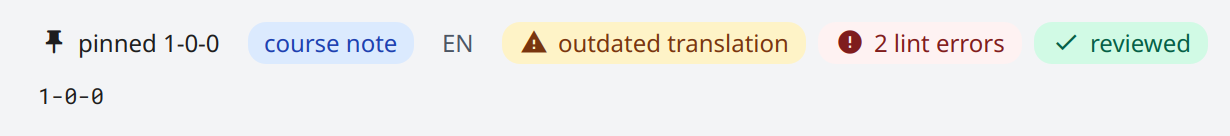
\includegraphics[width=\linewidth,height=0.11\textheight,keepaspectratio]{media/chip-light.png}\par\smallskip
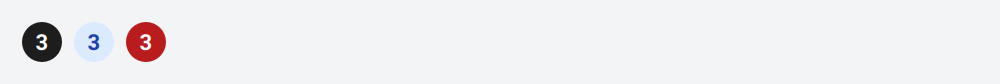
\includegraphics[width=\linewidth,height=0.11\textheight,keepaspectratio]{media/badge-light.png}\par\smallskip

\includegraphics[width=\linewidth,height=0.11\textheight,keepaspectratio]{media/label-light.png}\par\smallskip
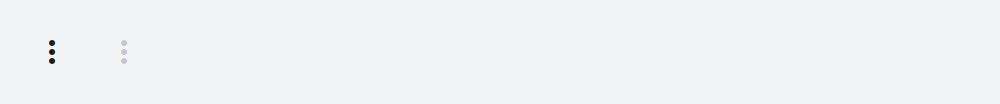
\includegraphics[width=\linewidth,height=0.11\textheight,keepaspectratio]{media/icon-button-light.png}\par\smallskip
\end{column}
\begin{column}{.48\linewidth}
\textbf{Dark}\par
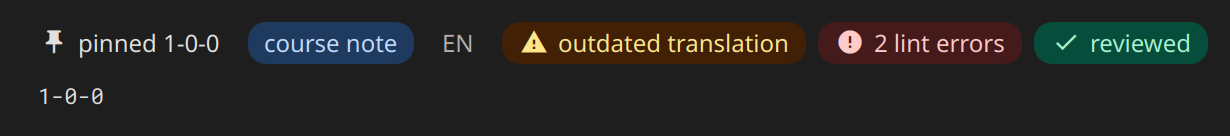
\includegraphics[width=\linewidth,height=0.11\textheight,keepaspectratio]{media/chip-dark.png}\par\smallskip

\includegraphics[width=\linewidth,height=0.11\textheight,keepaspectratio]{media/badge-dark.png}\par\smallskip

\includegraphics[width=\linewidth,height=0.11\textheight,keepaspectratio]{media/label-dark.png}\par\smallskip

\includegraphics[width=\linewidth,height=0.11\textheight,keepaspectratio]{media/icon-button-dark.png}\par\smallskip
\end{column}
\end{columns}
\begin{itemize}
\item Chip: compact metadata with semantic tones; \SMCode{mono=True} for versions or IDs. Badge: a small count/status.
\item Label roles: title, heading, body, caption. IconButton: compact action; \SMCode{set\_faint} gives interaction feedback.
\end{itemize}
\end{standardframe}
